\subsection{Backend and AS-Pair}\label{concept_BMC}

This chapter continues to work on the implementation from chapter \ref{conc_implement}. This involves a more in detail implementation of the MQTT interface as well as the backend and the database.

\subsubsection{Database schema}\label{database}

A database is needed to store information in a full stack system. However, this requires a predefined schema, as different schemas come into question depending on the database model, the structure of the data and the querying of the data. In this project, a relational database model will be used for a single backend connection.\\

In order to harmonize the collected data with the system presented in chapter \ref{concept}, the database schema from figure \ref{fig:database_schema} is used.\\

\begin{figure}[H]
    \centering
    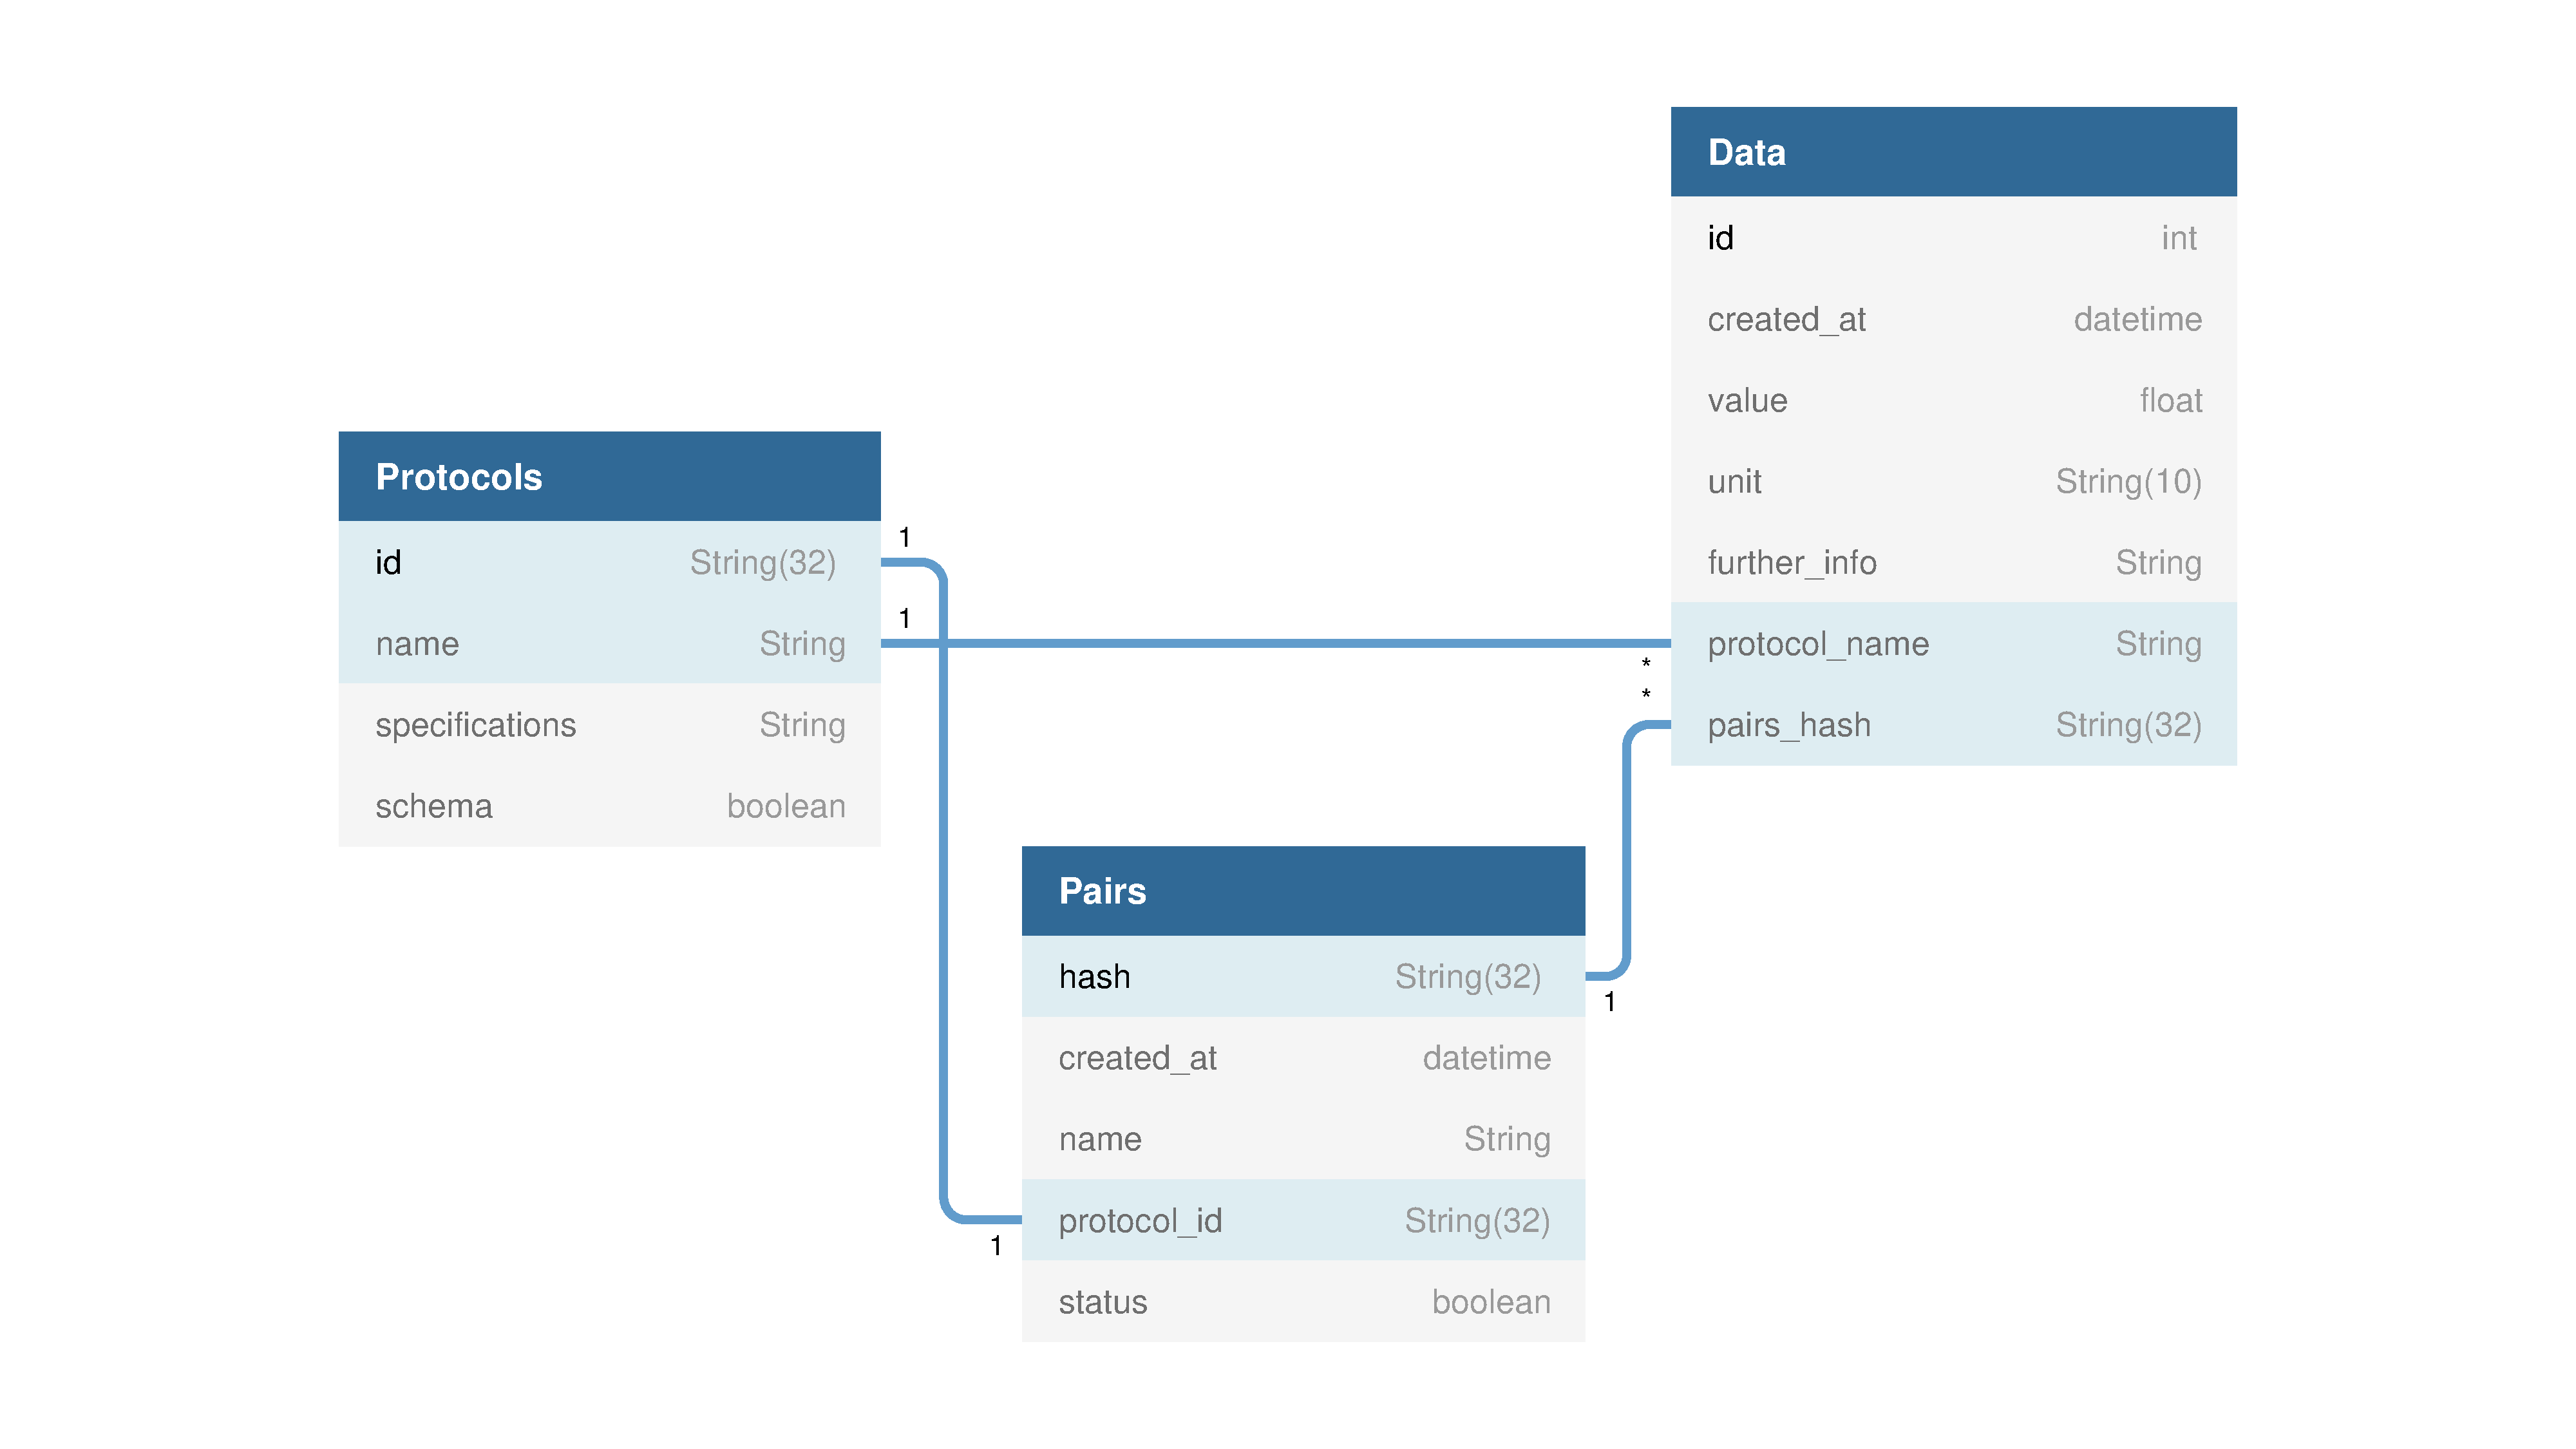
\includegraphics[width=.65\textwidth]{images/4_2/database_schema.pdf}
    \caption{Database schema}
    \label{fig:database_schema}
\end{figure}

Three tables are used for this: \textit{Pairs}, \textit{Protocol} and \textit{Data}. The Protocols and Data tables are assigned to the Pairs table. All registered pairs have a hash as a primary key, which is also stored on the AS-Pair. Each pair has one protocol that stores the parameters under which communication with the pair can take place. Furthermore, the boolean \textit{status} is used to distinguish whether an AS-Pair is still actively accessible via its interface.\\

\newpage

Protocols are again differentiated into registered and schematic protocols via the boolean \textit{schema}. Schematic protocols help the frontend to determine which interfaces are implemented in the backend and which additional information is required by the user to establish a connection to the AS-Pair via this interface. This additional information is stored in the protocol as the string \textit{specifications}. These can be dynamic for each interface.\\

Pairs can have a lot of data. Each data stores a \textit{value} from one sensor per AS-Pair with its \textit{unit} and, depending on how the interface is implemented, dynamically \textit{further information} about the sensor.


\subsubsection{Custom Messages}

MQTT is based on a publish/subscribe model, where data is sent between nodes via a topic to which other nodes are subscribed. It is important to note that data must not be sent on the same topic as the one on which data is received, as this can cause an infinite internal data exchange between nodes. This happens because the broker forwards all incoming data on a topic to all subscribed nodes. If nodes publish and subscribe on the same topic, they receive their own message back from the broker, which they send again on the same topic.\\

To prevent this, a custom messaging schema was developed for this project, which can be seen in figure \ref{fig:custom_msg}.

\begin{figure}[H]
    \centering
    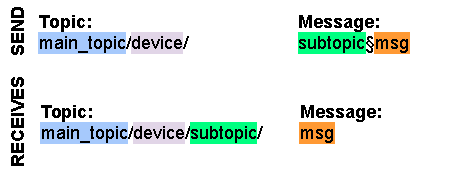
\includegraphics[width=.65\textwidth]{images/4_2/custom_msg.pdf}
    \caption{Custom messaging schema}
    \label{fig:custom_msg}
\end{figure}

If a node or the backend sends a message to another node the \textit{subtopic}, a special command to the AS-Pair which causes a specific reaction of the AS-Pair, is included in the message and separated from a possible message to the AS-Pair via a special character. The node or backend then subscribes to a joined topic, where the subtopic is included.\\

This means that the AS-Pair only has to be subscribed to one topic and can still differentiate all the subtopics sent. The node or the backend can ensure that only the desired AS-Pair will respond to the subtopic that is requested. In figure \ref{fig:custom_msg_ex_1} and figure \ref{fig:custom_msg_ex_2} one can see examples of implemented message exchanges.

\begin{figure}[H]
     \centering
     \captionsetup{justification=centering}
     \begin{minipage}[b]{0.5\textwidth}
         \centering
         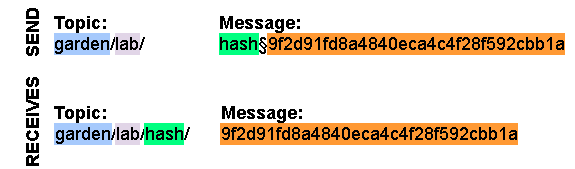
\includegraphics[width=\textwidth]{images/4_2/custom_example_1.pdf}
         \caption{Custom messages - Example 1}
         \label{fig:custom_msg_ex_1}
     \end{minipage}%
     \begin{minipage}[b]{0.5\textwidth}
         \centering
         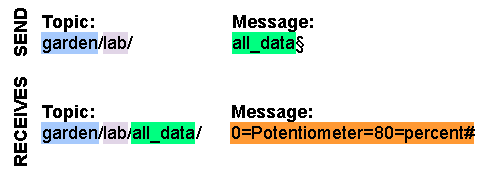
\includegraphics[width=\textwidth]{images/4_2/custom_example_2.pdf}
         \caption{Custom messages - Example 2}
         \label{fig:custom_msg_ex_2}
     \end{minipage}
\end{figure}


Figure \ref{fig:custom_msg_ex_2} is an example if several pieces of information have to be kept apart. In this case, information from sensors is decoded in a special pattern and sent to the requesting node or backend. The individual information and the individual information of the components are separated via special separating characters. It must be ensured that special separating characters are used that do not occur in possible values. The formatting of the message is the responsibility of the programmer of the interface.\\

In this example, information is requested from all sensors. The message received follows a strict specification: Individual sensors are separated via the \textit{\#}-character. In the segments, the ID of the sensor, its name, its value and its unit are then concatenated via the \textit{=}-character.\\

The same scheme is used to obtain all information about the implemented actuators. However, the content of the segments changes. The ID of the actuator, its name and its possible changeable variables with their data type are in this case returned.

\subsubsection{Routes}

For this project, 4 main workflows are to be implemented:  \textit{hash\_init}, \textit{get\_all\_data},\\ \textit{get\_actuator\_data} and \textit{set\_actuator}. These are shown and explained in the following figures.
\newpage

\begin{wrapfigure}{L}{0.55\textwidth}
    \centering
     \captionsetup{justification=centering}
     \begin{minipage}[b]{0.53\textwidth}
         \centering
         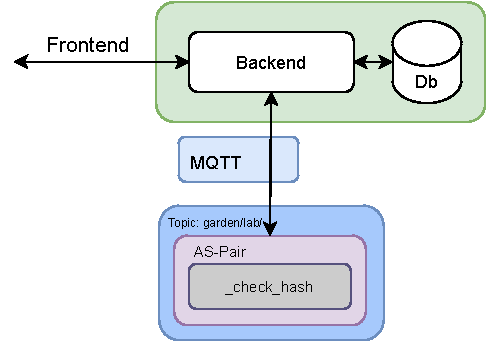
\includegraphics[width=\textwidth]{images/4_2_1/hash_init.pdf}
         \caption{Workflow \textit{hash\_init}}
         \label{fig:hash_init}
     \end{minipage}
     \vspace{-.25\baselineskip}
\end{wrapfigure}

\subsubsubsection{Initialize Hash}

In figure \ref{fig:hash_init} one can see the workflow of the \textit{hash\_init} route. The aim of this workflow is to register an AS-Pair in the backend.\\

For this purpose, the frontend sends a request to the backend with information about the AS-Pair, such as its name, which interface is to be used and what information is needed to establish a connection with the AS-Pair. For MQTT, this would be the IP of the broker and the topic of the AS-Pair. This allows the backend to attempt to establish communication with the AS-Pair. \\

The Backend, however, checks beforehand whether there is already a similar AS-Pair in the database. If such an AS-Pair with the given specifications is already specified in the database, it is reactivated if it if no connection has been established in a longer period of time, i.e. its flag \textit{status} is set to True, or a message is returned to the frontend that the sent AS-Pair already exists and is active. This avoids duplicate entries from the same AS pair.\\

If a communication has been successfully established with the AS-Pair under the subtopic hash, the AS-Pair checks whether it has already saved a hash. For this purpose, it receives from the backend either a newly generated hash, if no database entry exists, or an already registered hash, if an entry in the database exist with the same specifications.\\

If the AS-Pair was able to save the hash successfully, positive feedback is sent back with the hash as the message, which the backend stores with all relevant data in the database and sends a positive message back to the frontend.\\

\begin{wrapfigure}{L}{0.43\textwidth}
    \centering
     \captionsetup{justification=centering}
     \begin{minipage}[b]{0.39\textwidth}
         \centering
         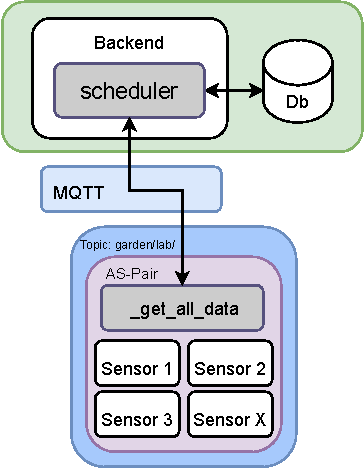
\includegraphics[width=\textwidth]{images/4_2_1/scheduler_all_data.pdf}
         \caption{Workflow \textit{get\_all\_data}}
         \label{fig:schedule}
     \end{minipage}
     \vspace{-.25\baselineskip}
\end{wrapfigure}

\newpage

\subsubsubsection{Scheduler}

In figure \ref{fig:schedule} one can see the workflow of the \textit{hash\_init} route. The aim of this workflow is to store the value from all initialized sensors of all registered AS-Pairs in the database at periodic intervals.\\

For this purpose, the backend needs a scheduled task that queries all active AS-Pairs from the database in a fixed interval and attempts to establish a communication with this AS-Pairs over their specified communication specifications. \\

Since numerous AS-Pairs can be registered and individual requests may exceed the interval time, depending on the selected interval time, these communications must take place in asynchronous threads. This way, individual requests do not block each other and several requests can be processed simultaneously over the I/O Interfaces.\\

These requests are made under the subtopic \textit{data\_all} to all active AS-Pairs. Through this subtopic, the AS-pair returns all data from all initialized sensors. The developer of the interface can decide how he wants to save the result of the sensors into the database through the column \textit{further information}. However, two values must be stored per data-row in the table data, i.e. per sensor: The value of the sensor and the unit of this value.\\

\begin{wrapfigure}{L}{0.43\textwidth}
    \vspace{\baselineskip}
    \centering
     \captionsetup{justification=centering}
     \vspace{-4mm}
     \begin{minipage}[b]{0.39\textwidth}
         \centering
         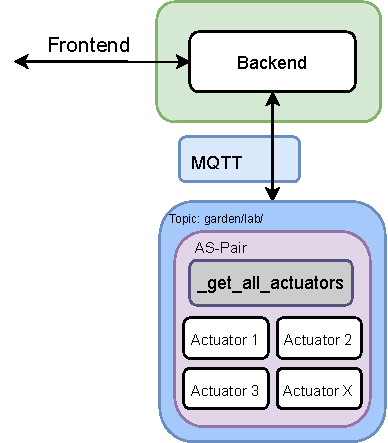
\includegraphics[width=\textwidth]{images/4_2_1/get_actuator.pdf}
         \caption{Workflow \textit{get\_actuator\_data}}
         \label{fig:get_act}\par
         \vspace{9mm}
         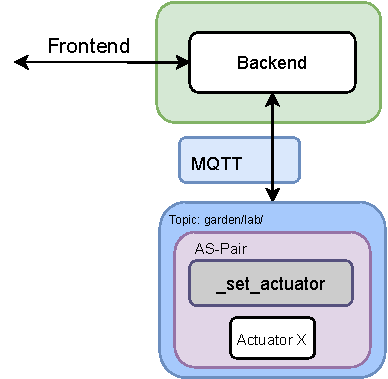
\includegraphics[width=\textwidth]{images/4_2_1/set_actuator.pdf}
         \caption{Workflow \\\textit{set\_actuator}}
         \label{fig:set_act}
     \end{minipage}
     \vspace{-.25\baselineskip}
\end{wrapfigure}

\subsubsubsection{Get and set Actuator}

In figure \ref{fig:get_act} and \ref{fig:set_act} one can see the workflows of the \textit{get\_actuator\_data} and \textit{set\_actuator}. The aim of the overall workflow is to control a registered Actuator of an AS-Pair. This requires information about the actuators and their changeable variables, as well as an interface with which a specific actuator can be controlled.\\

\newpage

For this purpose, the frontend sends a request to the backend with information about which AS-Pair it would like to receive information about its actuators. The backend sends a request via the interface under the subtopic \textit{actuator\_all} to the specified AS-Pair.\\

The AS-pair sends back a list of all initialized actuators in a special way: ID of the actuator, its name and its possible changeable variables with their data type. The changeable variables depend on the implementation of the actuator. \\

This information is sent back to the frontend. From this information, the frontend or the user can now send a request to the backend to change the variables mentioned in the reply.\\

For this purpose, the frontend sends a message to the backend with the information which actuator ID is to be controlled at which AS-Pair and the variables with their new values.\\

The backend communicates with the specified AS-Pair via it's interface and communicates the new information. If the actuator was successfully controlled with the new values, the AS-Pair sends a positive message to the backend, which returns a positive message to the frontend. \\

In the event of an error, the error message is communicated to the frontend via the backend.

